\section{Test on simulated data}\label{results}
In this section, we test our new approach with Coordinate Descent on simulated MeerKAT data. We show that our approach does not need to calculate the whole Fourier Transform matrix $F$. Instead, we use a heuristic to only use relevant columns. As mentioned in section \ref{cd}, it is unknown if our approach will converge to the true optimum. Nevertheless, we compare our results with CASA's CLEAN implementation, and demonstrate super-resolution performance of Coordinate descent together with accurate total flux modelling.

The two simulated datasets contains idealized MeerKAT observations. Compared to the real world, the two simulated datasets contain few Visibilities and not representative of the real data volume. Also, more realistic simulations which contain pointing-, calibration-, and thermal noise are out of scope for this project. The simulations are used to isolate the two fundamental issues in radio interferometer image reconstruction: Non-uniform sampling and incomplete measurements.

\subsection{Super-resolution of two point sources}
The first simulated observation contains two non-zero pixels, i.e. point sources, with intensity of 2.5 and 1.4 Jansky/Beam. The image has a size of $256^2$ at a resolution of 0.5 arc-seconds per pixel. The integral, the total Flux of the image, is 3.9 Jansky/beam.

\begin{figure}[h]
	\centering
	\begin{subfigure}[b]{0.4\linewidth}
		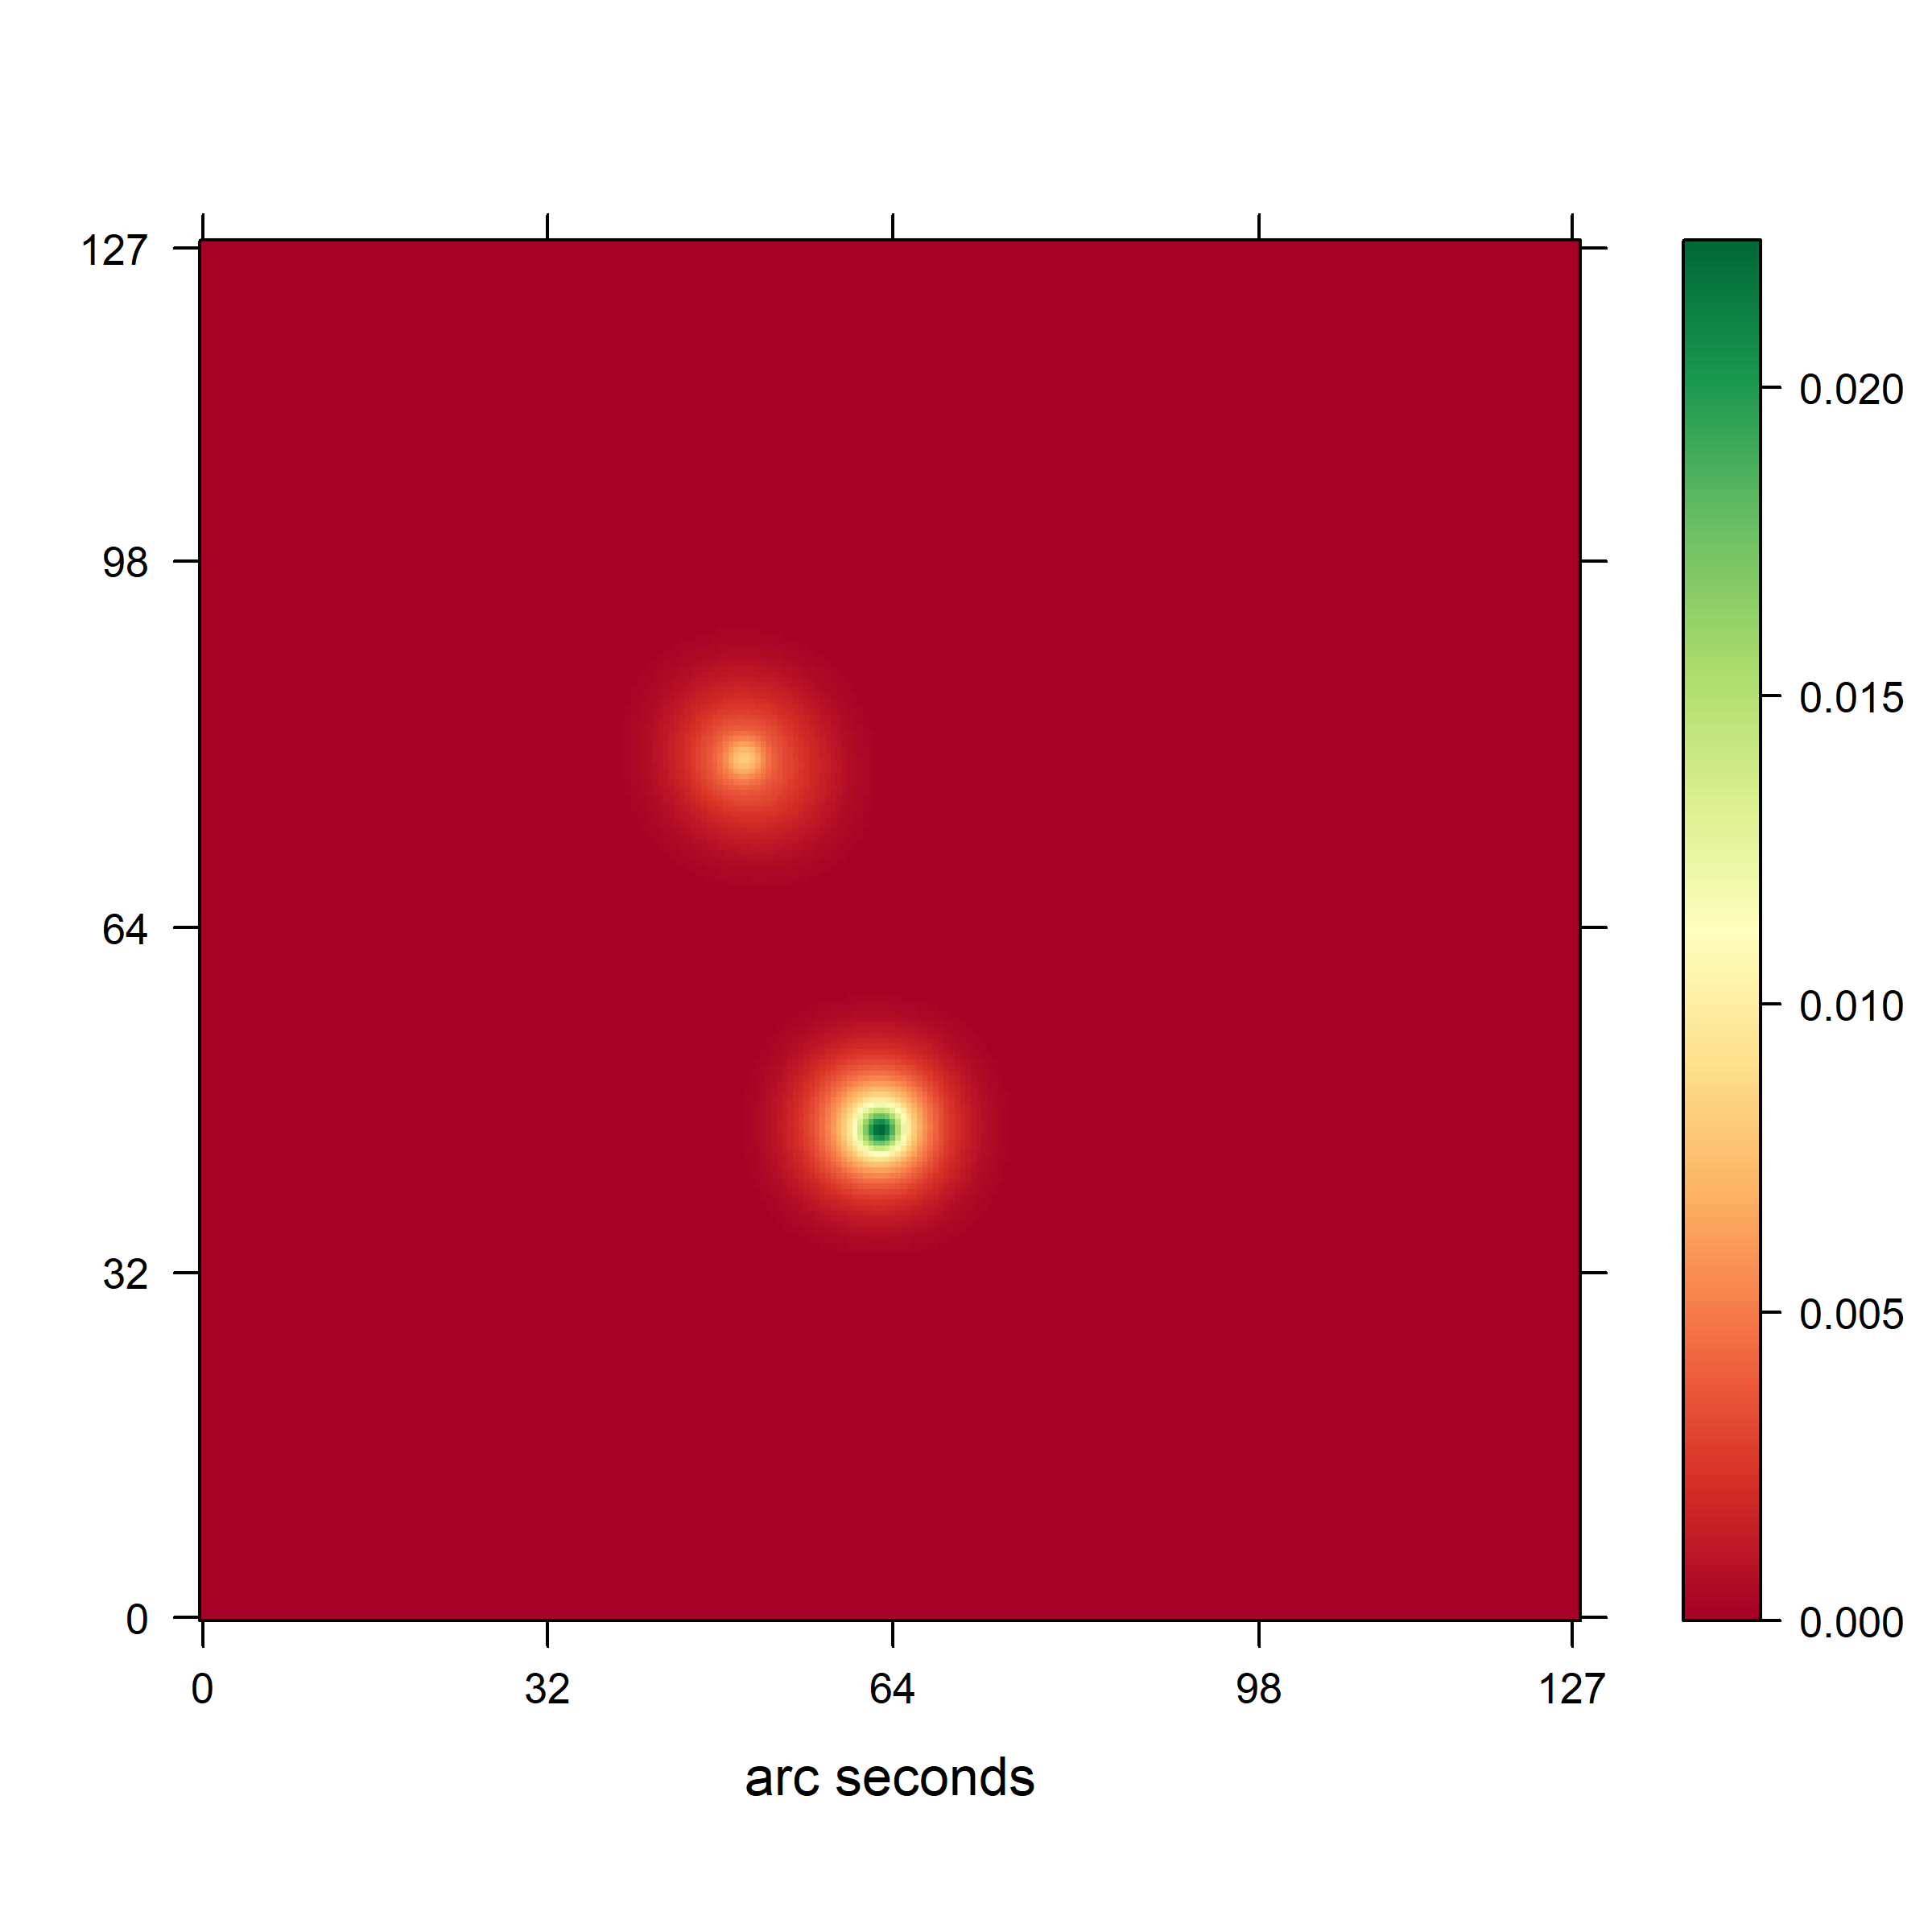
\includegraphics[width=\linewidth, trim={0.2in, 0.2in, 0, 0.2in}, clip]{./chapters/20.results/points/tclean_points.png}
		\caption{CLEAN reconstruction \\with CASA standard parameters.}
		\label{results:points:tclean}
	\end{subfigure}
	\begin{subfigure}[b]{0.4\linewidth}
		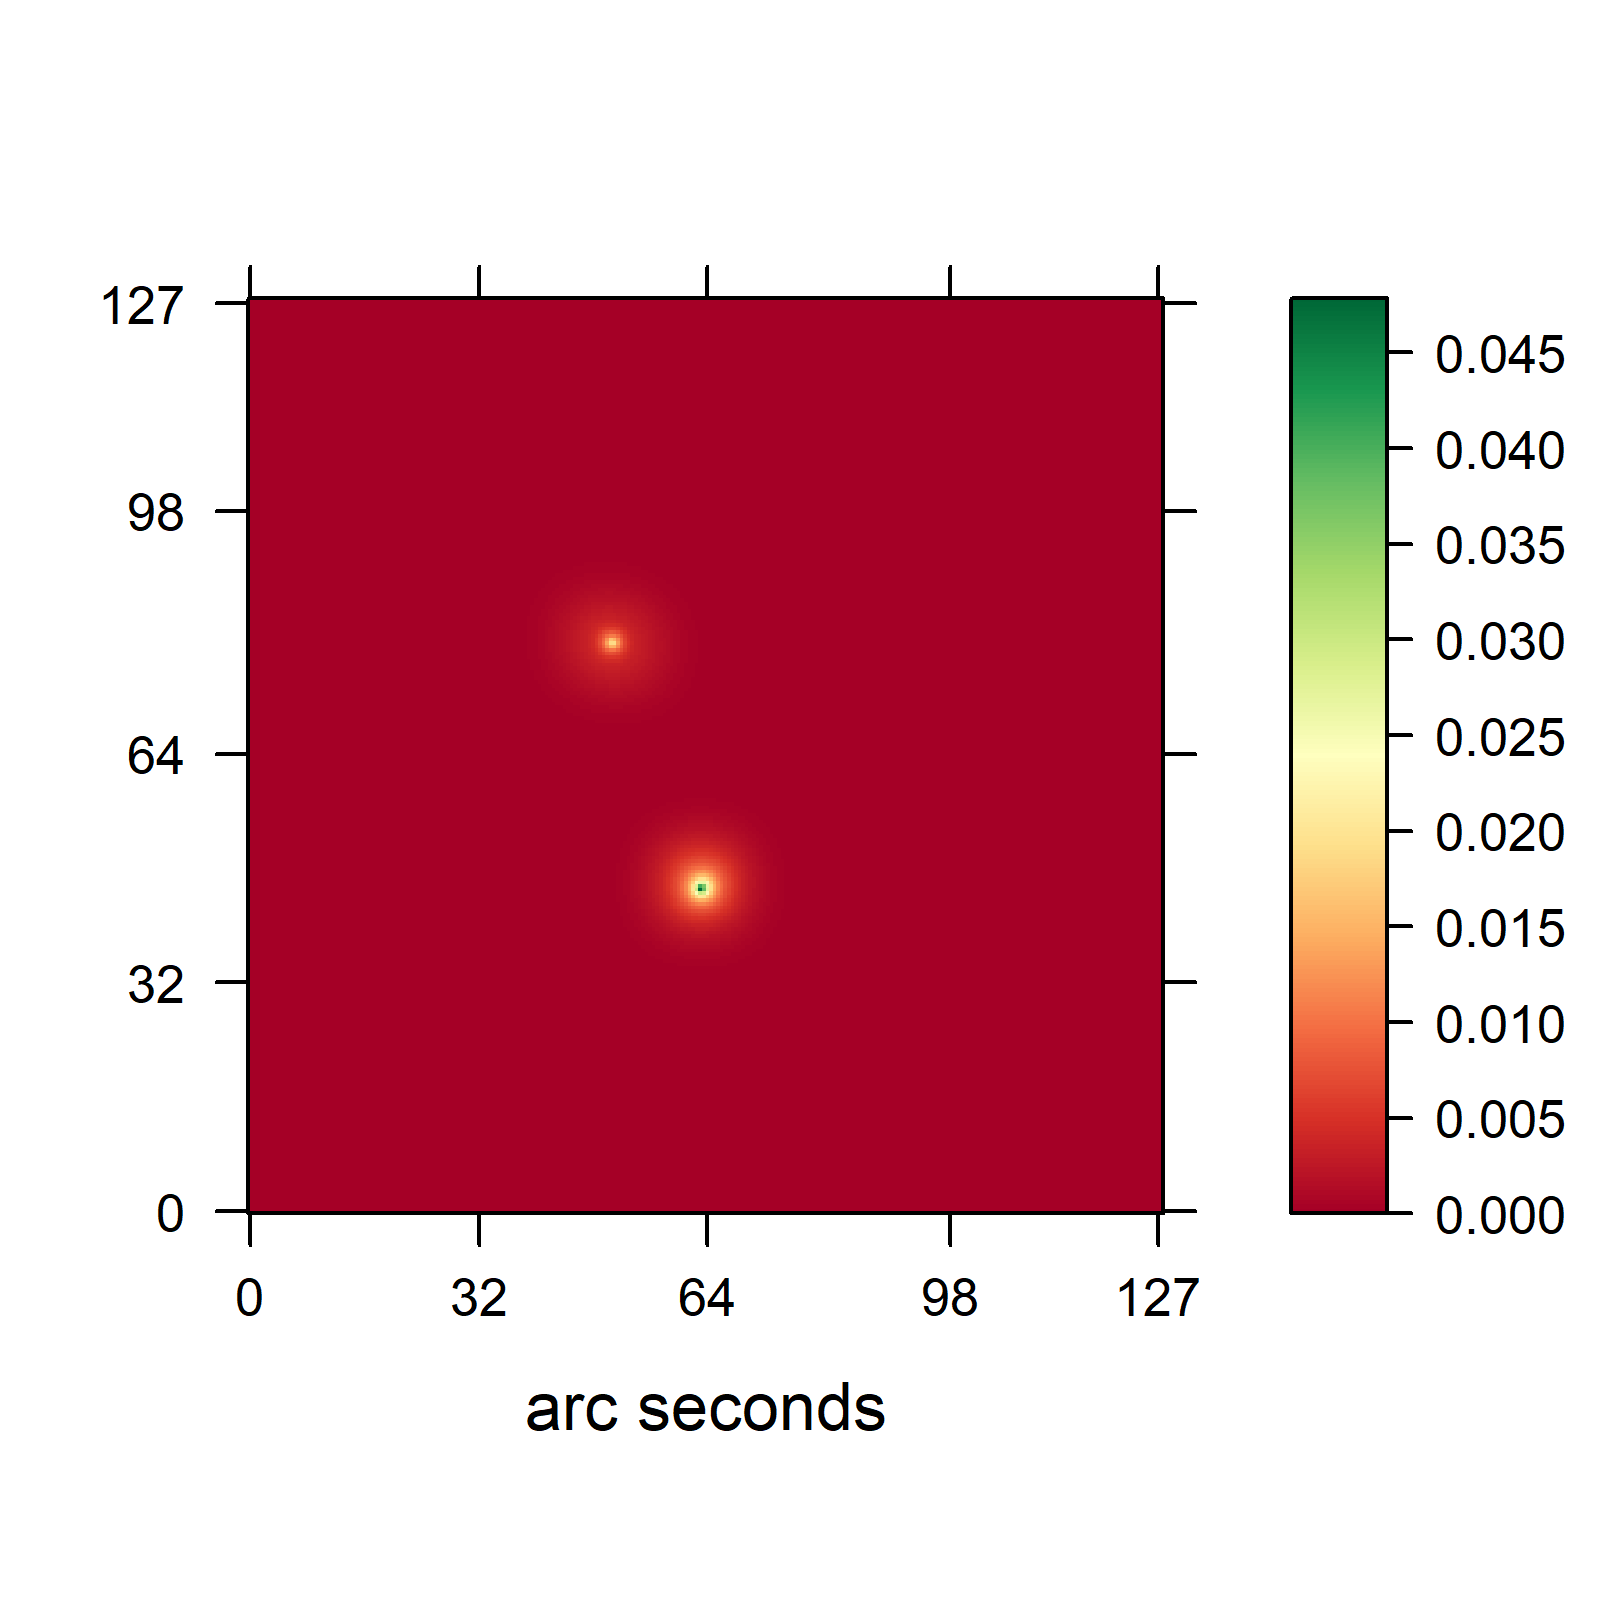
\includegraphics[width=\linewidth, trim={0.2in, 0.2in, 0, 0.2in}, clip]{./chapters/20.results/points/cd_points.png}
		\caption{Coordinate Descent reconstruction\\ with $\lambda = 0.01, J=4$.}
		\label{results:points:cd}
	\end{subfigure}
	
	\caption{Image reconstruction of two simulated point sources.}
	\label{results:points}
\end{figure}

The figure \ref{results:points} shows the CLEAN and the Coordinate Descent reconstruction. CLEAN reconstructs the image \ref{results:points:tclean} at the accuracy limit of the instrument. It essentially reconstructs a blurred version of the observed image, where the blurring represents the accuracy of the instrument. With compressed sensing, we aim to reconstruct the de-blurred image, increasing the effective accuracy of the instrument. 

Coordinate Descent in image \ref{results:points:cd} shows a super-resolved reconstruction of the two point sources. It reconstructs two narrow peaks surrounded,by a low-intensity Gaussian emission. Also, Coordinate Descent manages to capture the total flux more accurately than CLEAN.  The total flux of image \ref{results:points:cd} results in 3.92 Jansky/beam, compared to CLEAN which overshoots the number by a factor of 1400. The total flux of the CLEAN reconstruction \ref{results:points:tclean} overshoots the 3.9 figure by a factor of 1400. This gets obvious when we compare the intensity profile of CLEAN, Coordinate Descent and the ground truth in figure \ref{results:points:contour}.

\begin{figure}[h]
	\centering
	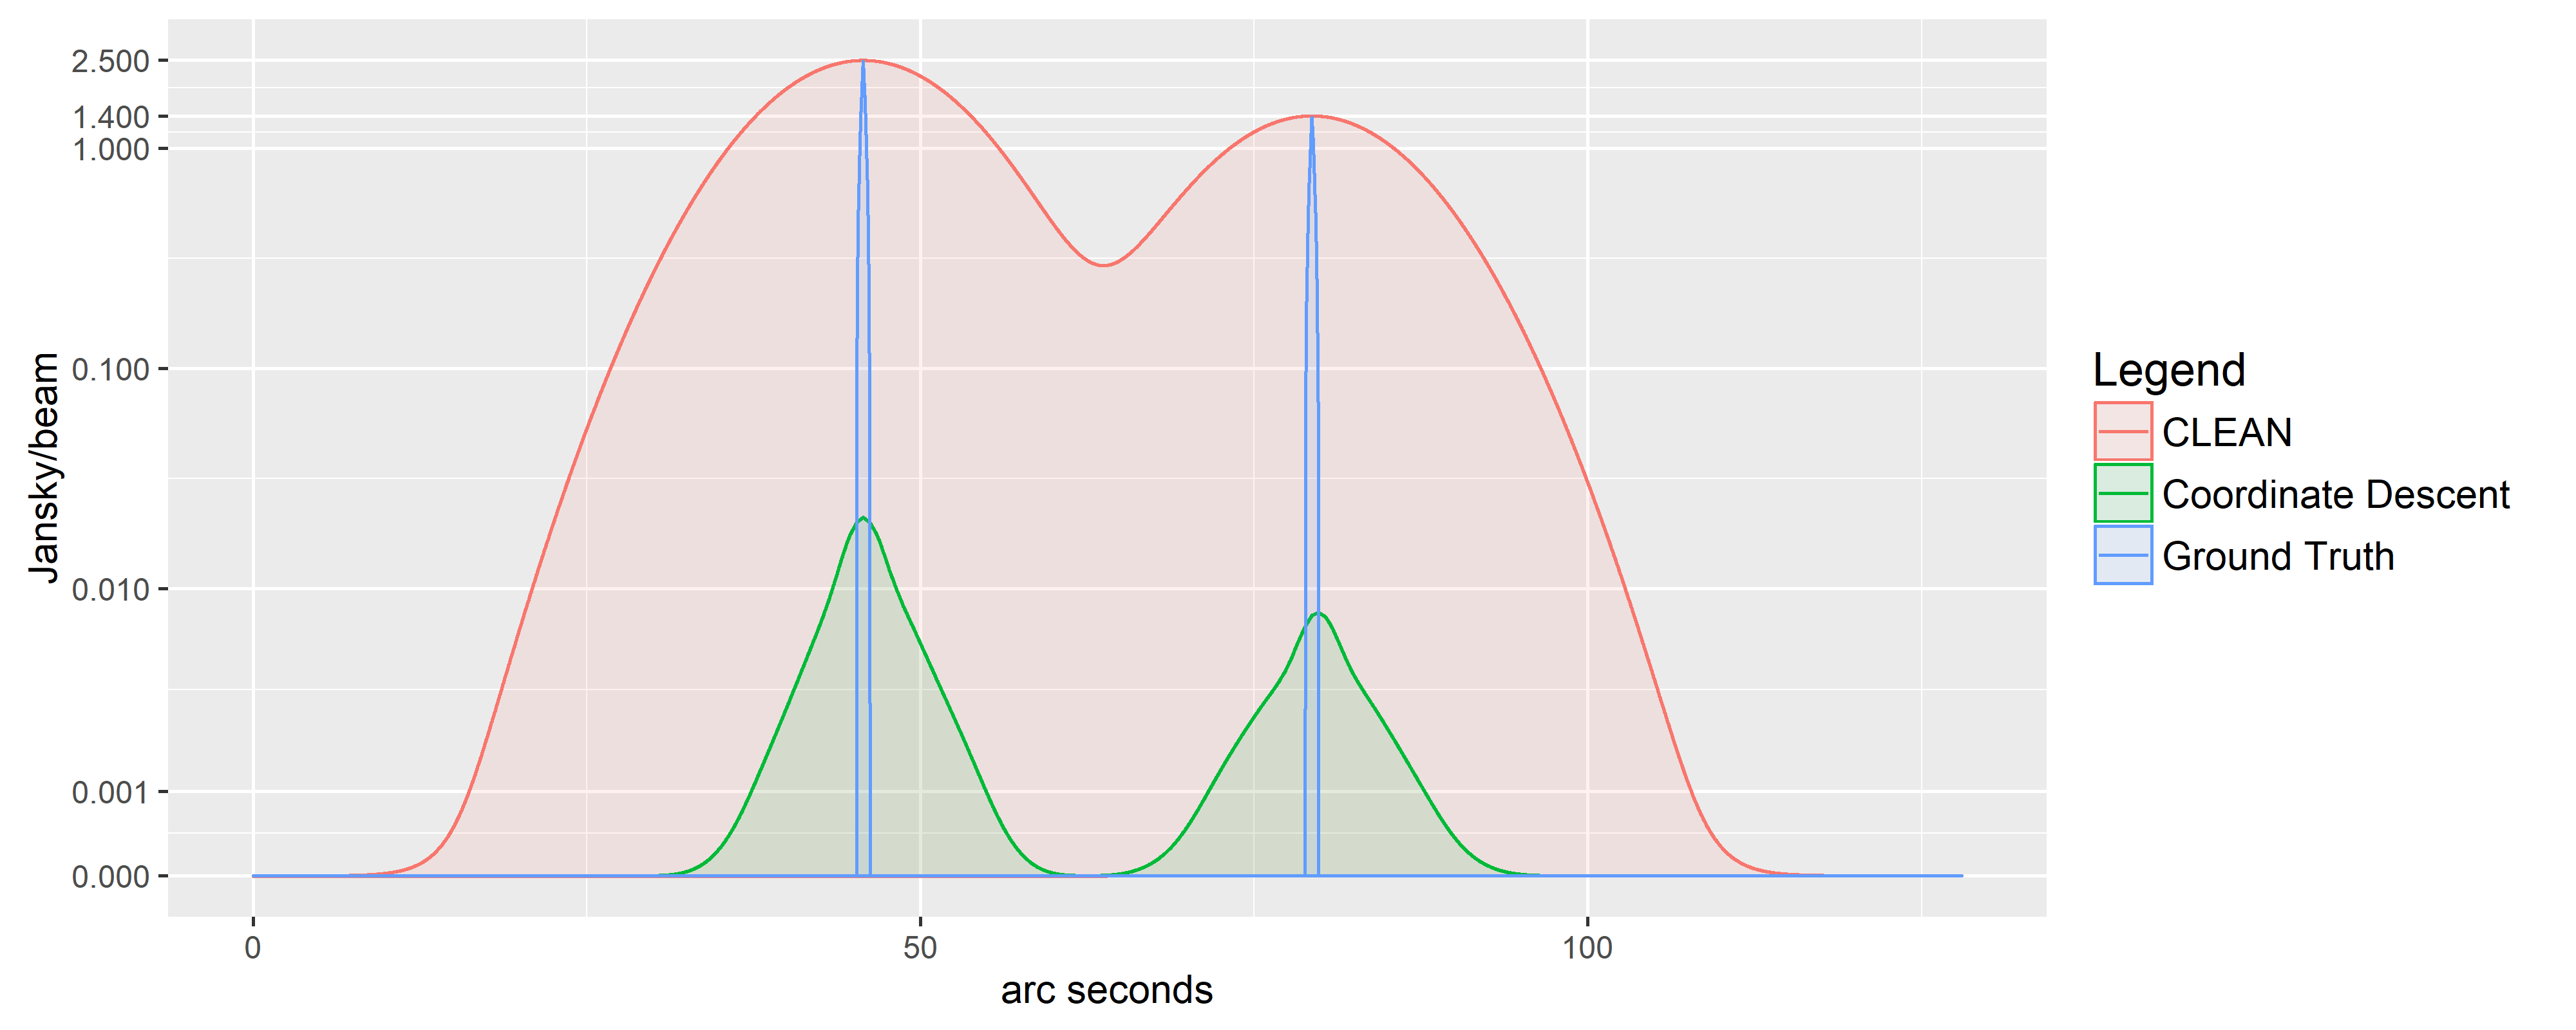
\includegraphics[width=0.8\linewidth]{./chapters/20.results/points/contour_points.png}
	\caption{Intensity profile of the two point sources.}
	\label{results:points:contour}
\end{figure}

CLEAN essentially places a Gaussian function with correct peak intensity at the point source location, but it does not respect the total flux of the image. Coordinate Descent keeps the total flux in mind. The pixels in each area of the point sources sum up to the correct values of 2.5 and 1.4 respectively. However, note that Coordinate Descent in figure \ref{results:points:contour} seems to have both point sources shifted by approximately a pixel. It looks suspiciously like an off-by one error. Sadly in the time frame of this project, no error was found or an explanation for this behaviour.

%Possible 

\subsection{Super resolution of mixed sources}
This dataset contains a mixture of three Gaussian emissions and sixteen point sources of varying intensities. At the center of the image, it has three point sources underlying a weak extended emission. The image center and one Gaussian emissions are analysed in detail. Coordinate Descent was run for two full iterations, using  $\lambda=0.01$ and $J=7$ starlet layers. The CLEAN and Coordinate Descent reconstructions are shown in figure \ref{results:mixed}. Our algorithm was able to locate the point sources below the accuracy limit of MeerKAT. However, some point sources were reconstructed with artefacts.

\begin{figure}[h]
	\centering
	\begin{subfigure}[b]{0.4\linewidth}
		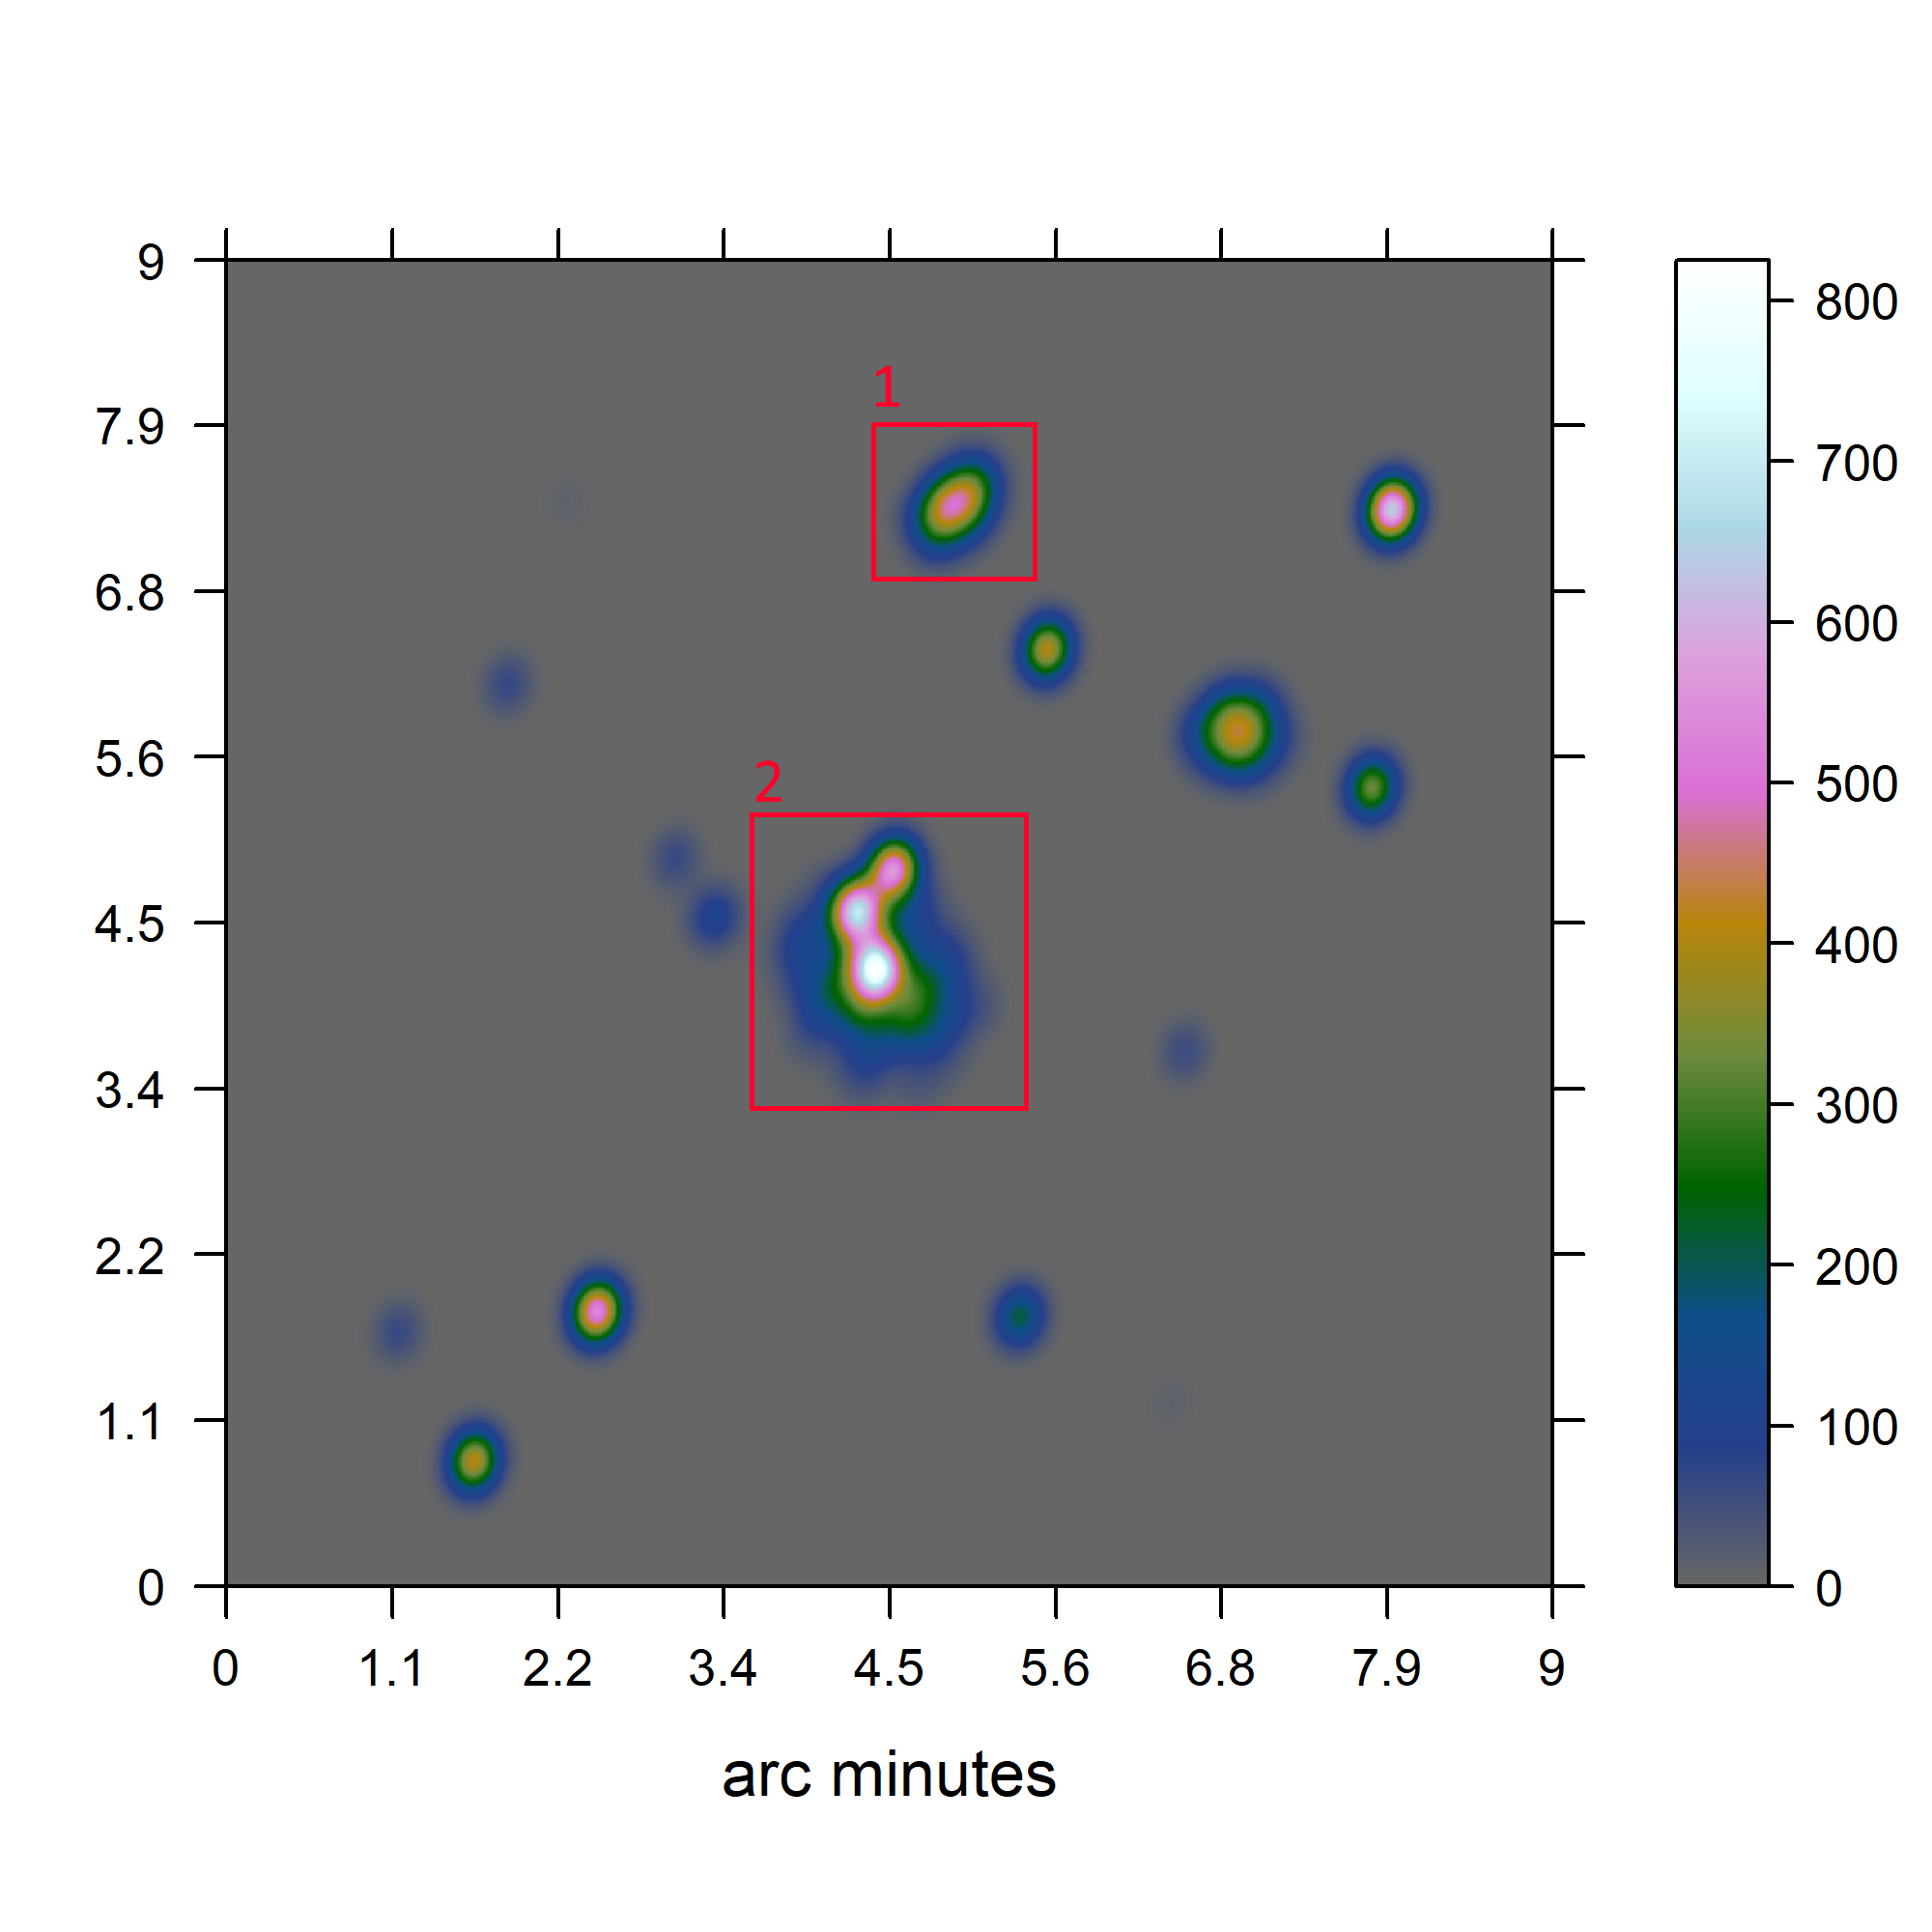
\includegraphics[width=\linewidth, trim={0.2in, 0.2in, 0, 0.2in}, clip]{./chapters/20.results/mixed/mixed_clean_boxed.png}
		\caption{CLEAN reconstruction}
		\label{results:mixed:tclean}
	\end{subfigure}
	\begin{subfigure}[b]{0.4\linewidth}
		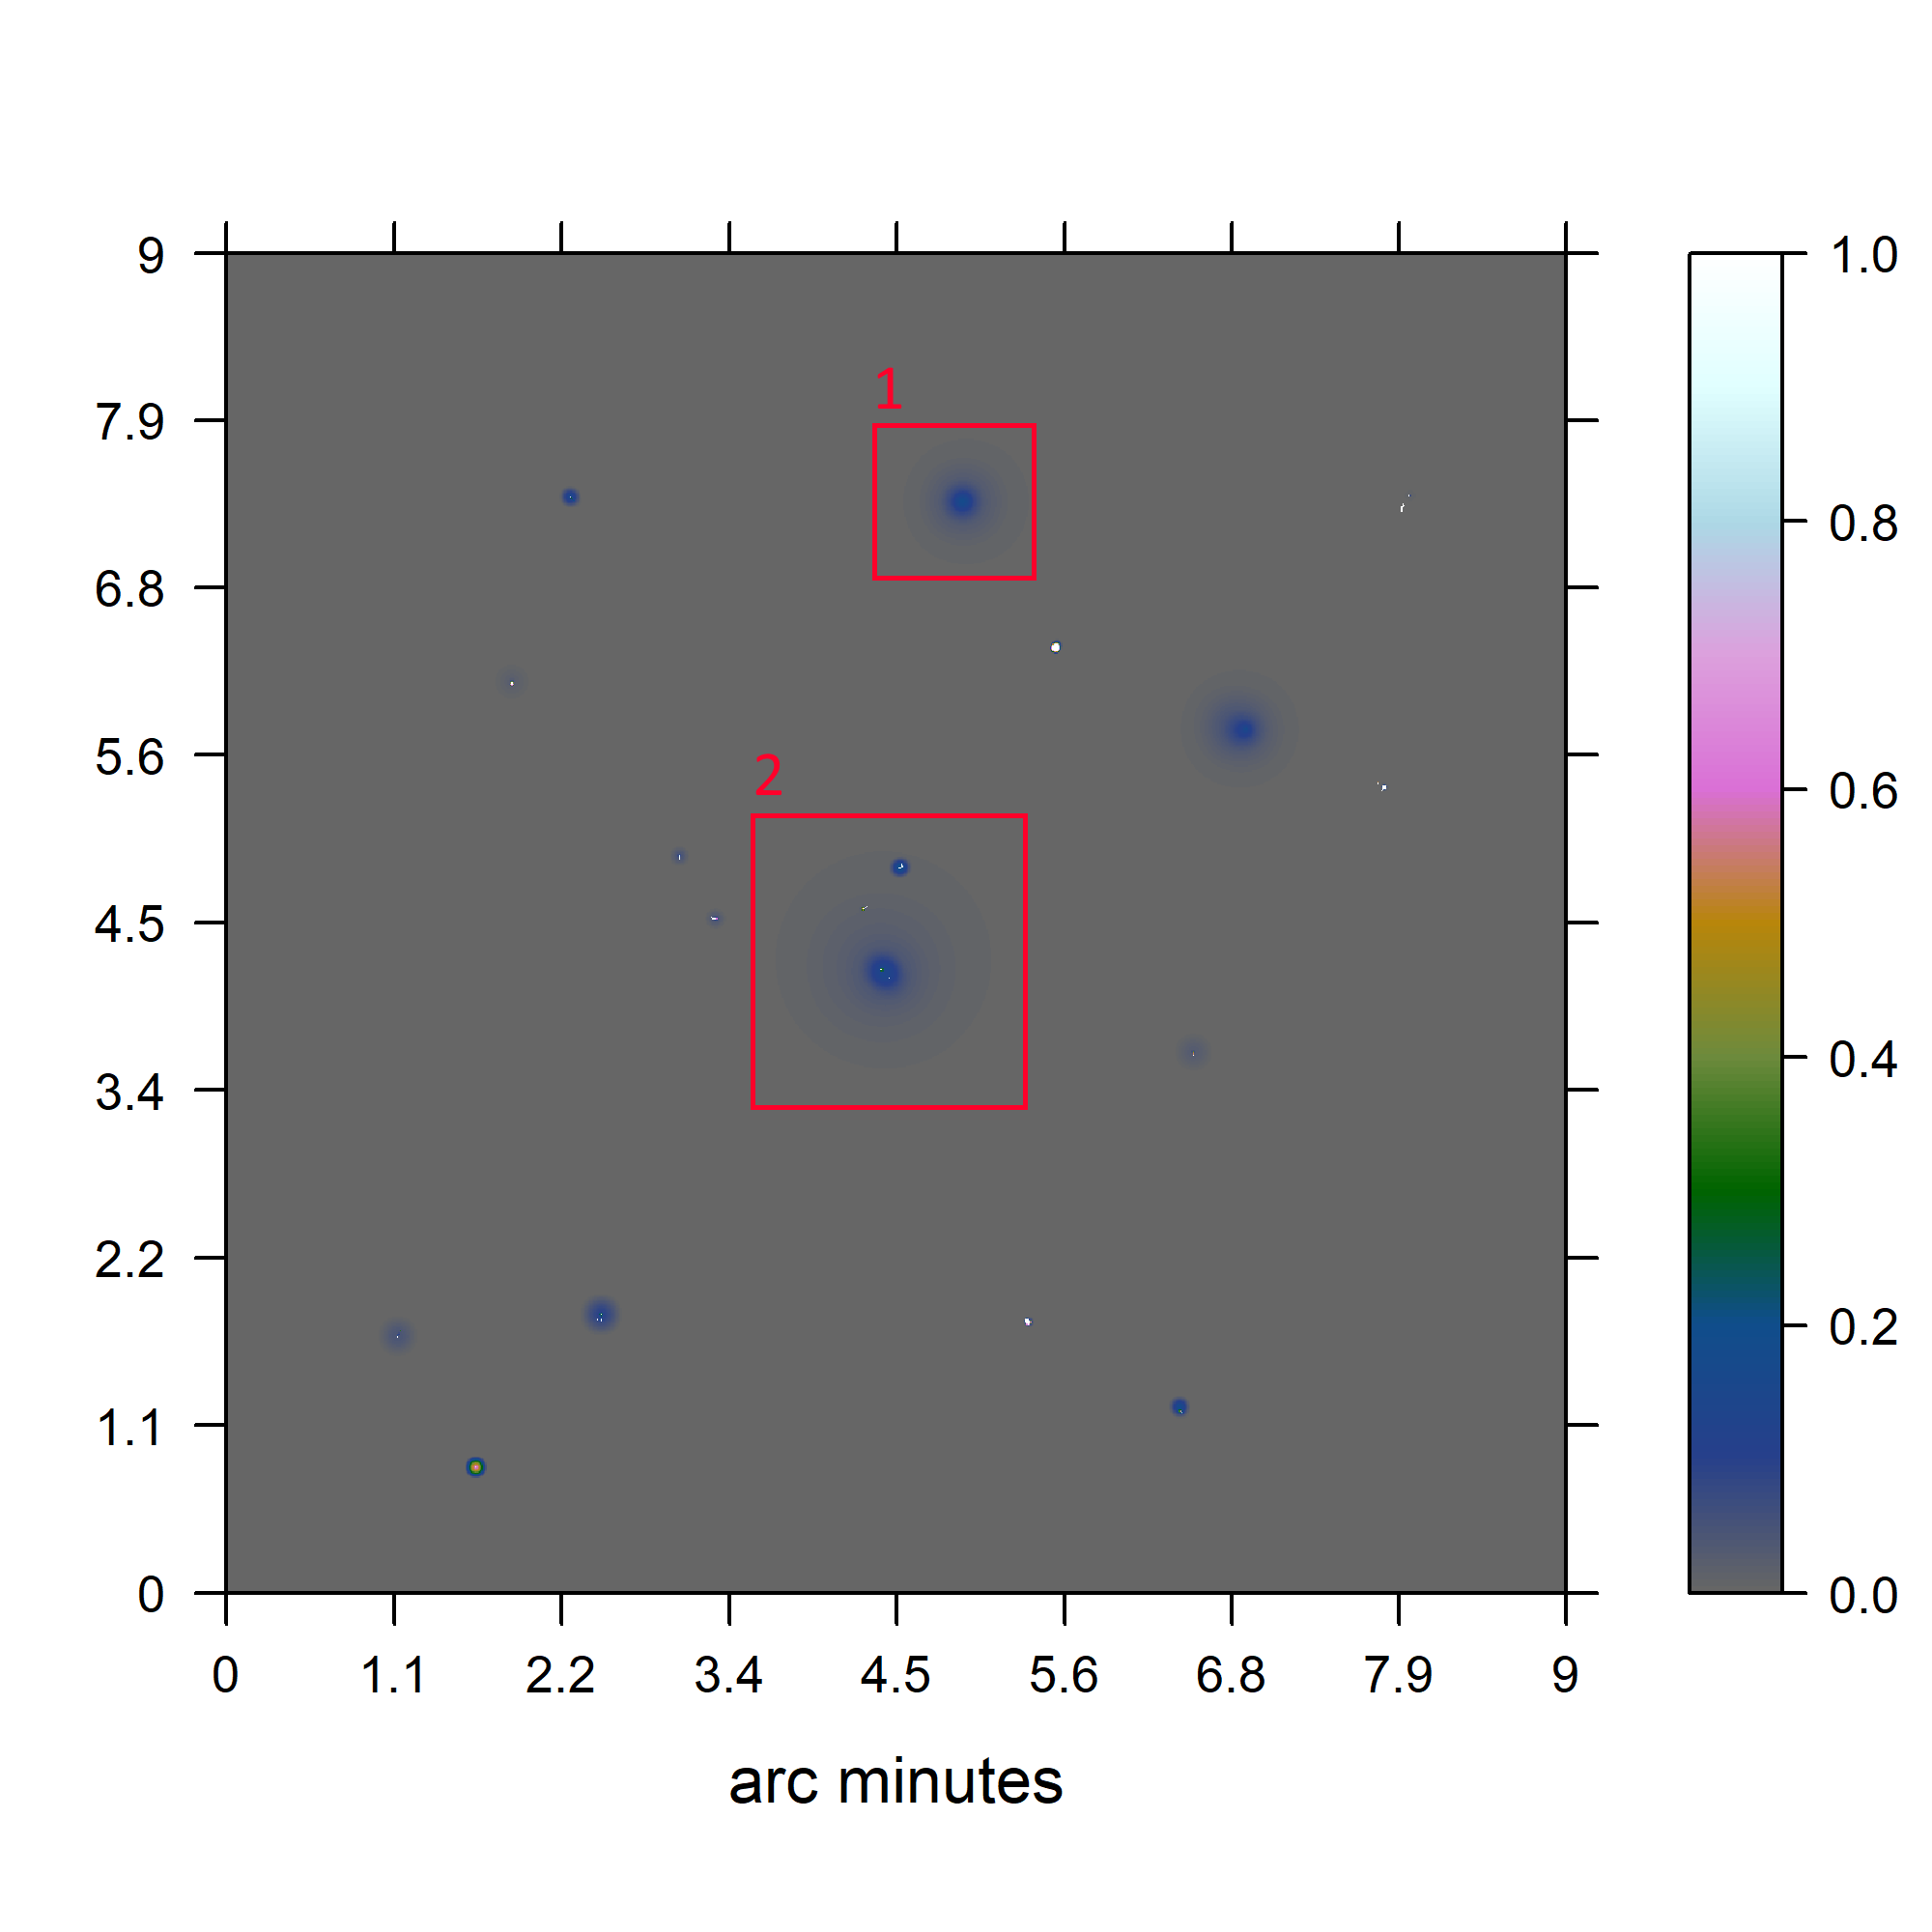
\includegraphics[width=\linewidth, trim={0.2in, 0.2in, 0, 0.2in}, clip]{./chapters/20.results/mixed/mixed_cd_boxed.png}
		\caption{Coordinate Descent Reconstruction}
		\label{results:mixed:cd}
	\end{subfigure}
	\caption{Reconstruction on mixed sources}
	\label{results:mixed}
\end{figure}

The number of Fourier columns scales with the number of non-zero components




Question of Flux reconstruction



\begin{figure}[h]
	\centering
	\begin{subfigure}[b]{0.3\linewidth}
		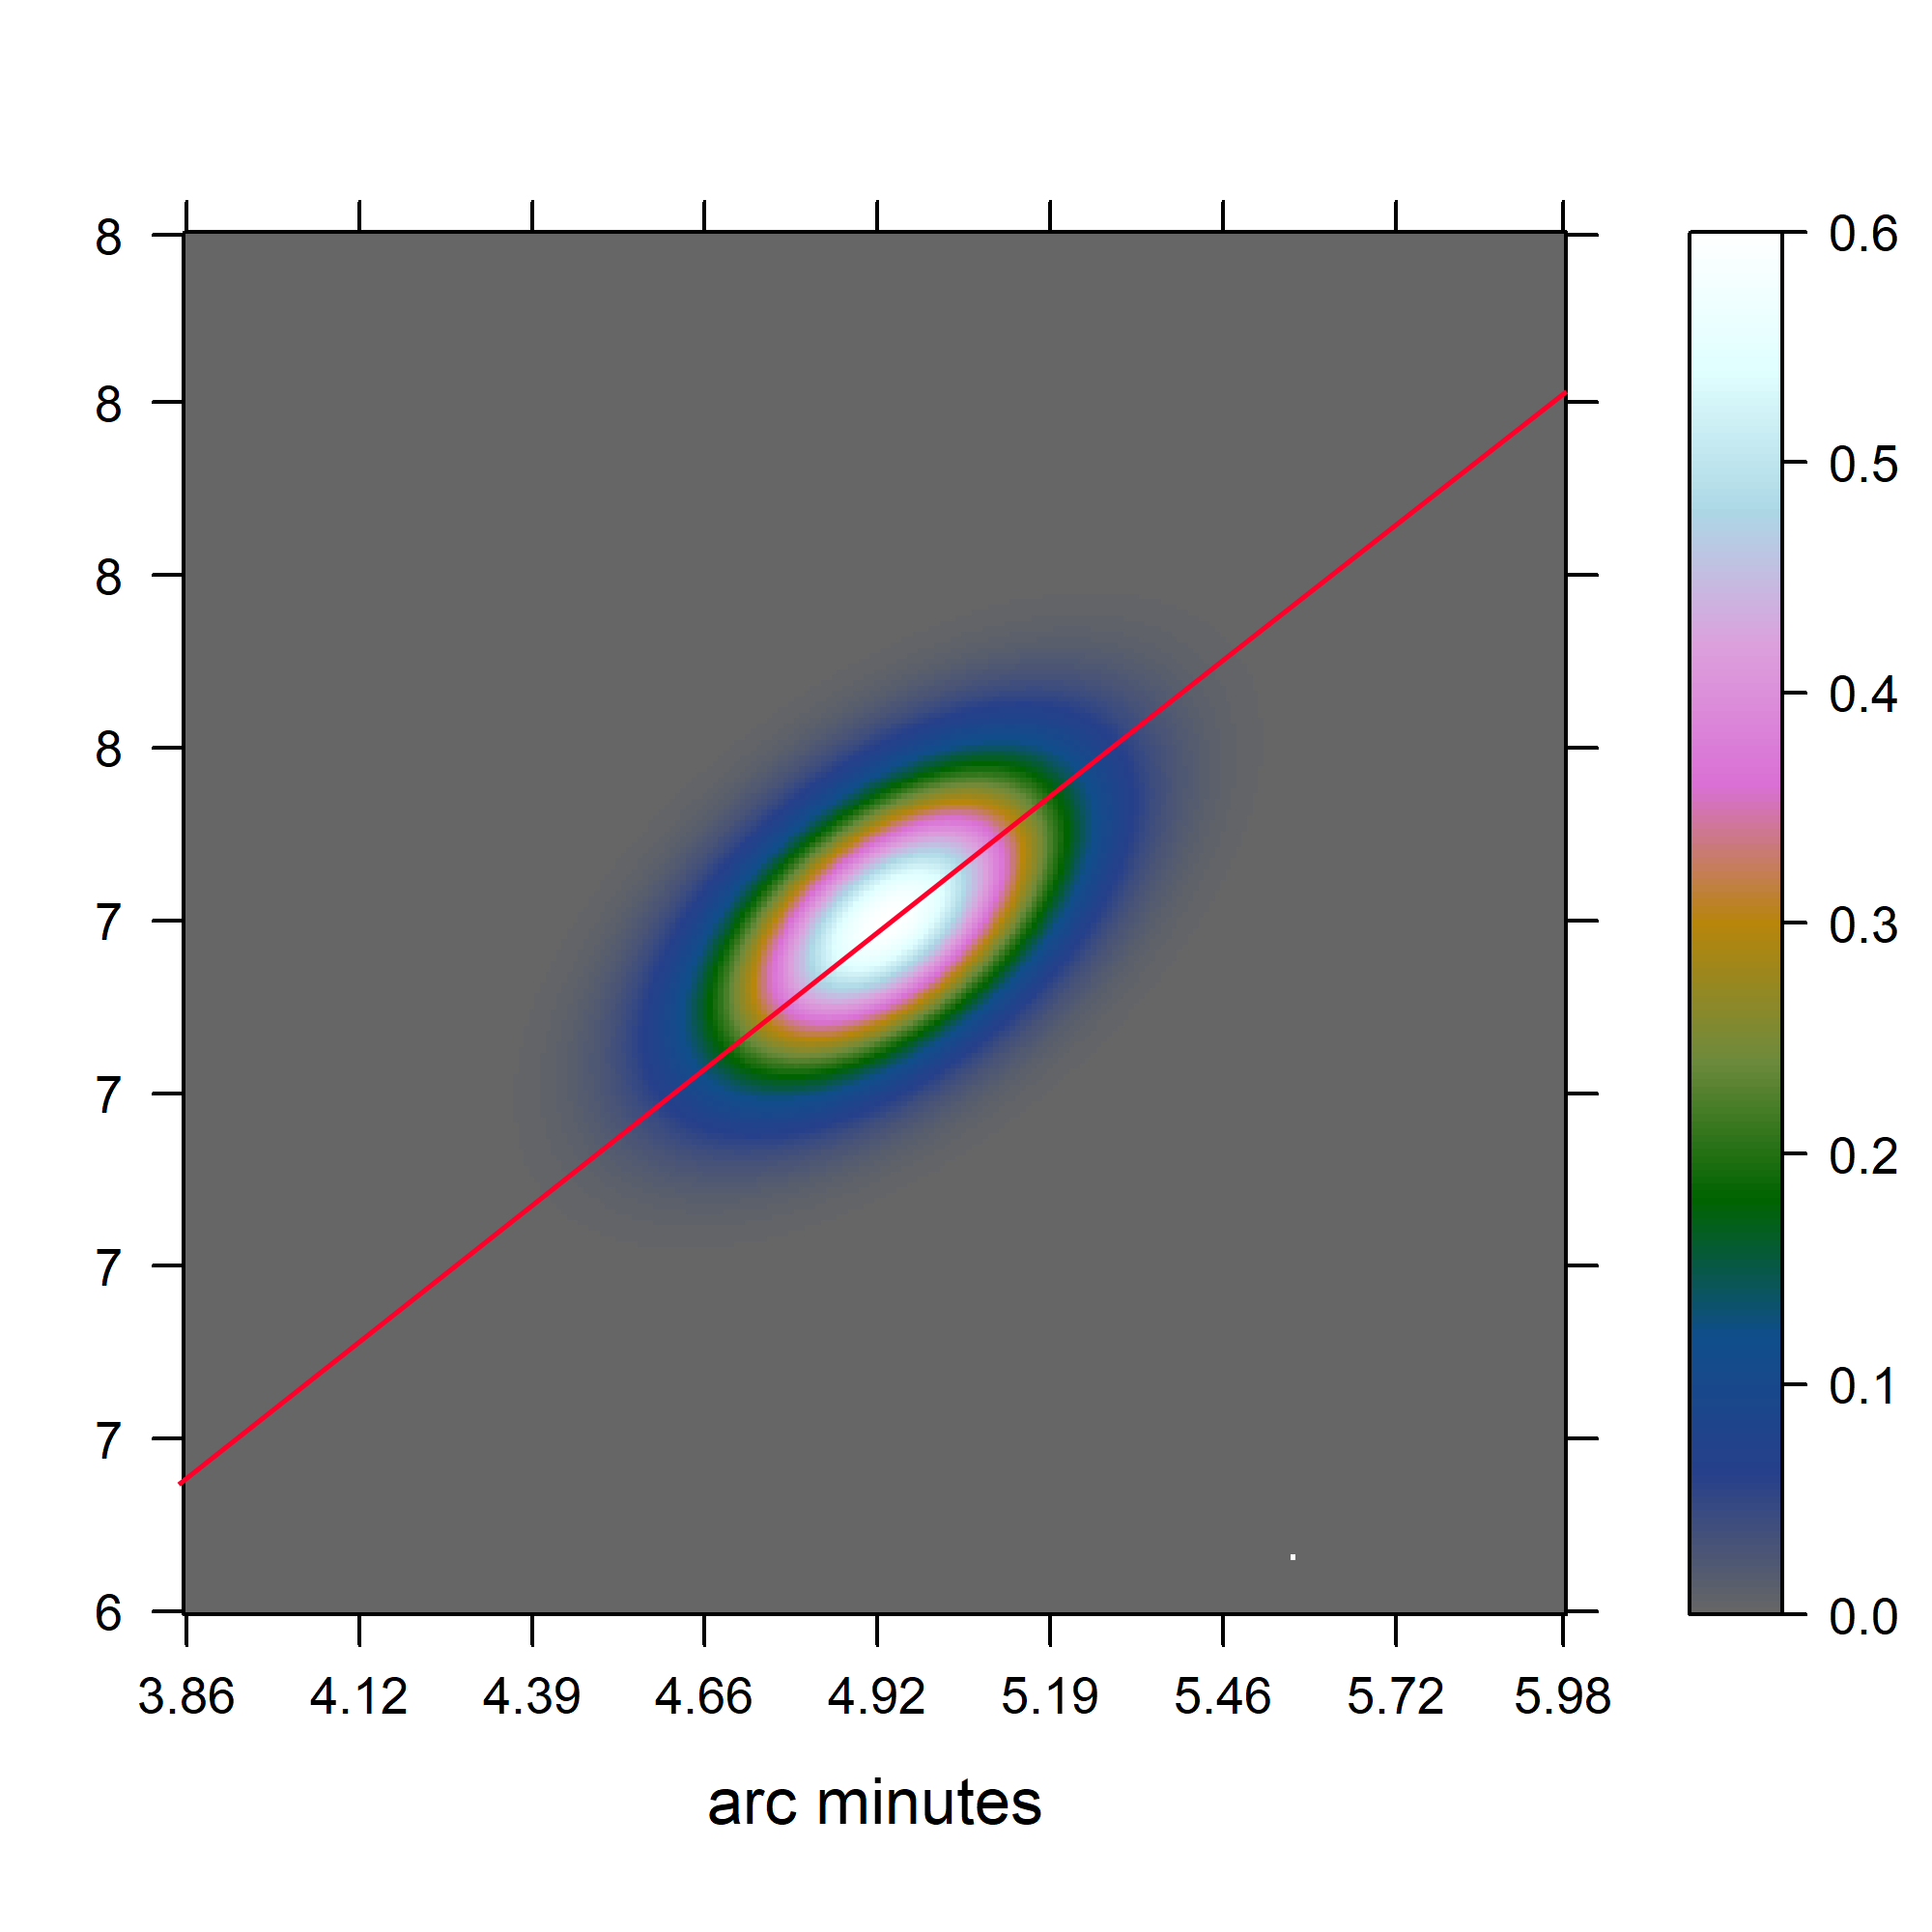
\includegraphics[width=\linewidth, trim={0.4in, 0.9in, 3.2in, 1.8in}, clip]{./chapters/20.results/mixed/mixed_cut_model_line.png}
		\caption{Ground truth.}
		\label{results:mixed:cut0:img}
	\end{subfigure}
	\begin{subfigure}[b]{0.6\linewidth}
		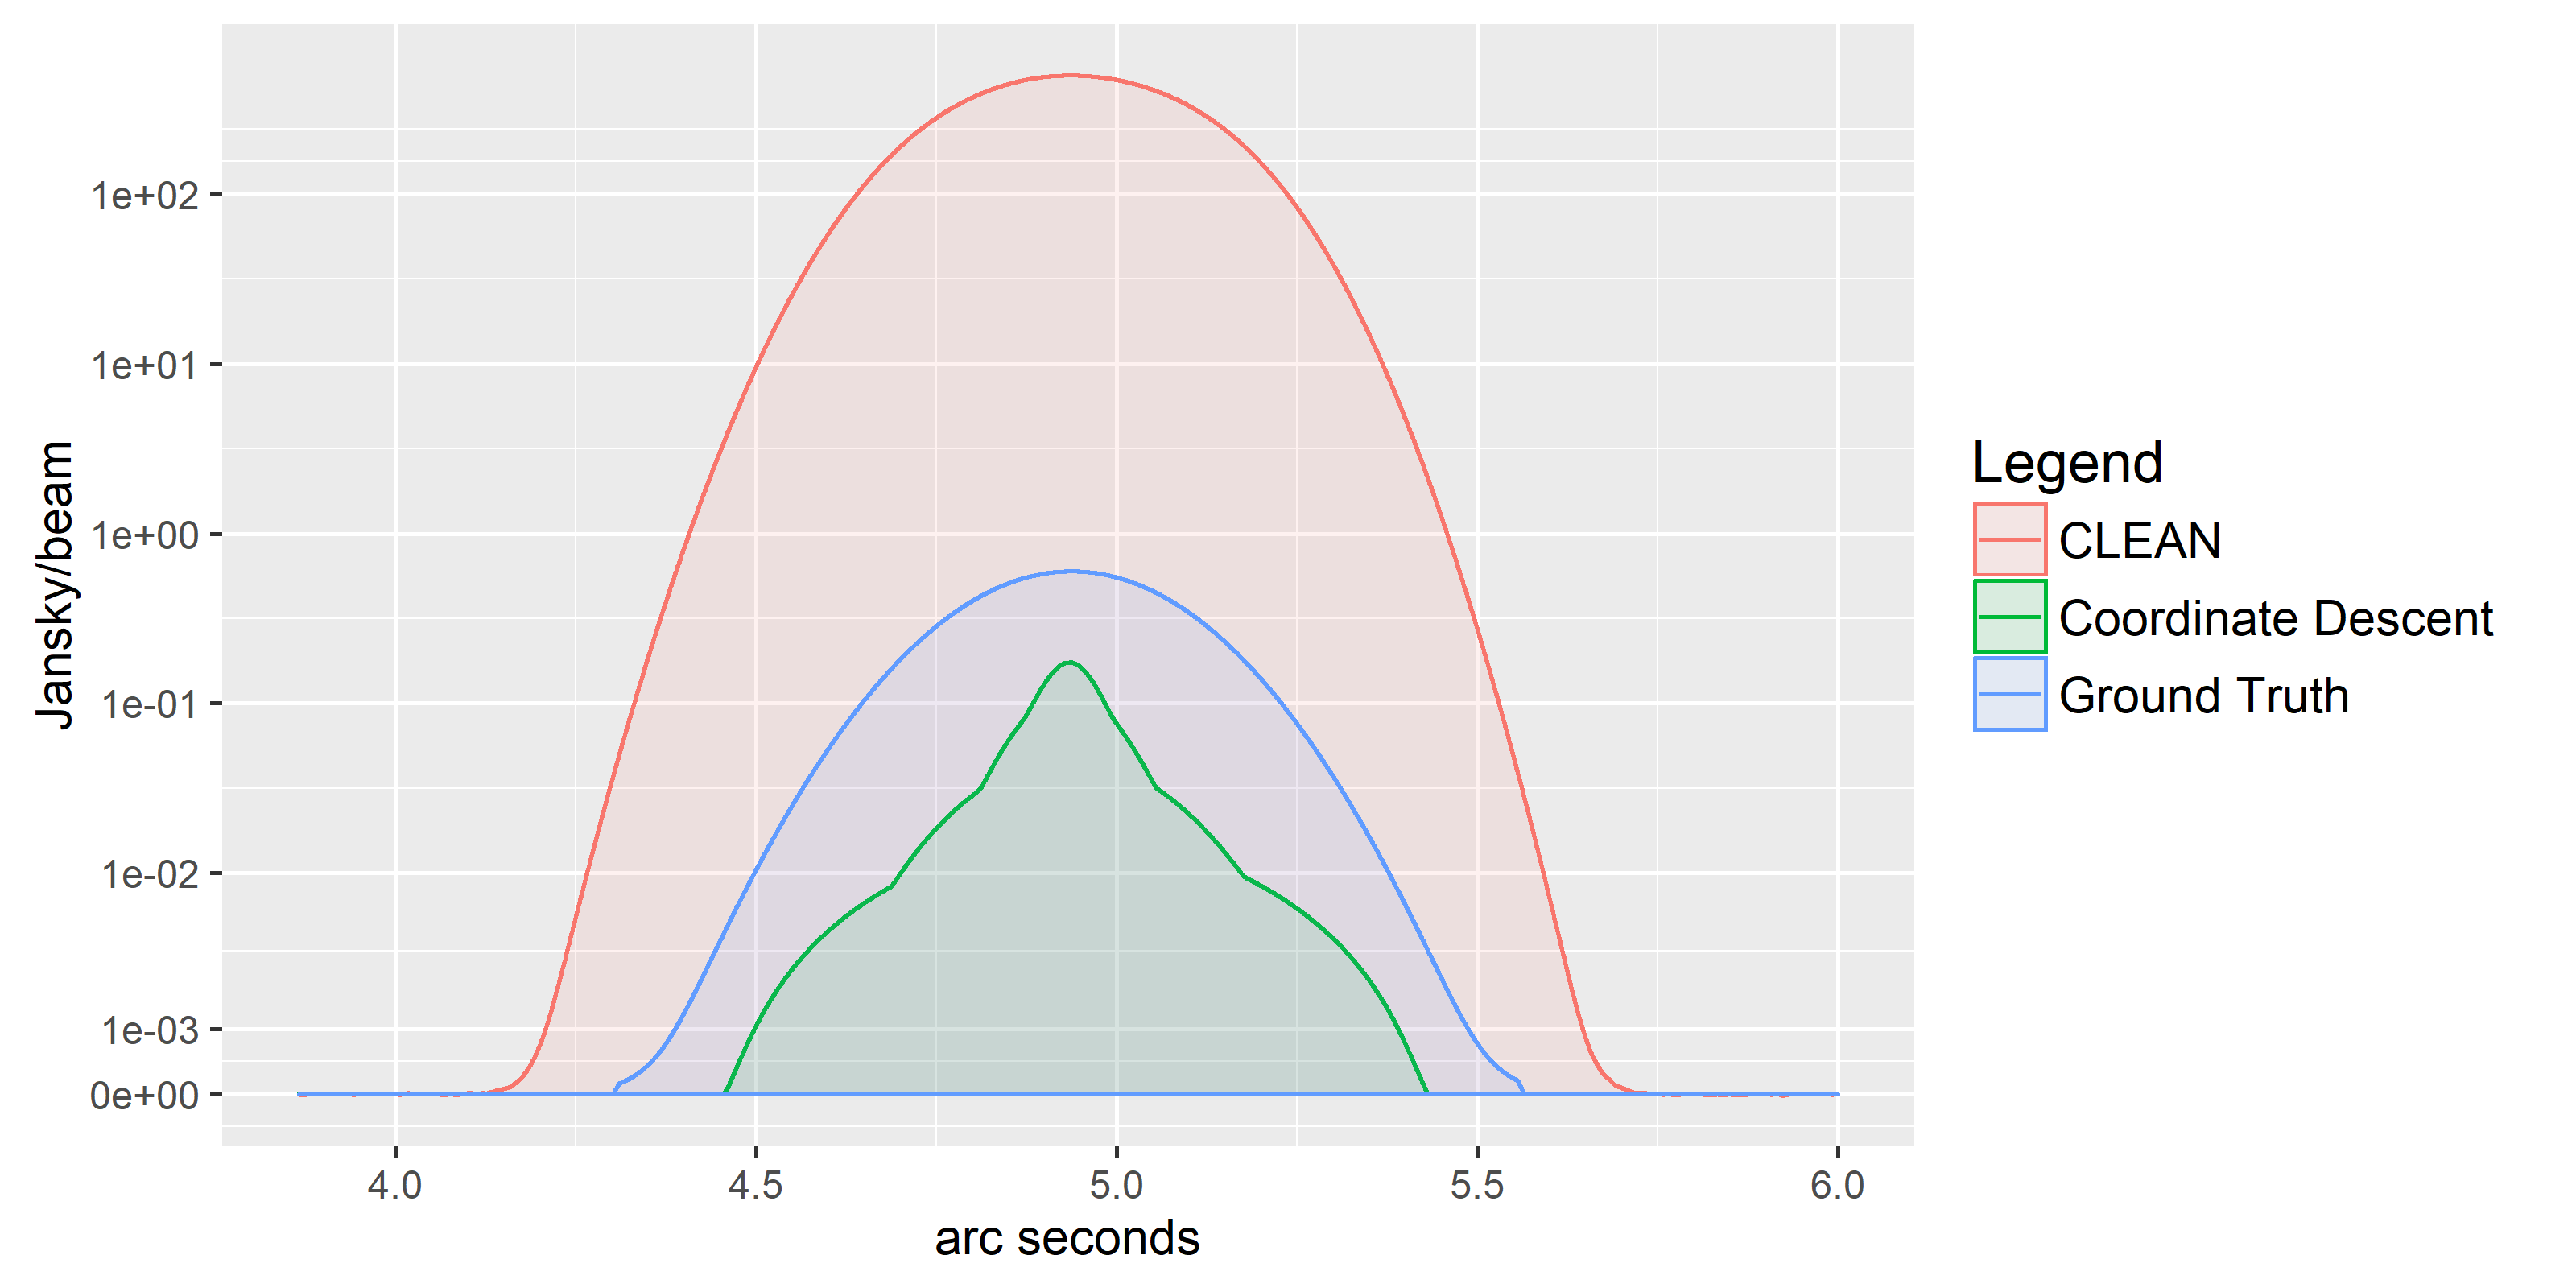
\includegraphics[width=\linewidth, trim={0, 0, 0.2in, 0.2in}, clip]{./chapters/20.results/mixed/mixed_cut0.png}
		\caption{Intensity profile.}
		\label{results:mixed:cut0:profile}
	\end{subfigure}
	\caption{Intensity profile of region 1.}
	\label{results:mixed:cut0:contour}
\end{figure}

More accurate total flux reconstruction, but no

\begin{figure}[h]
	\centering
	\begin{subfigure}[b]{0.3\linewidth}
		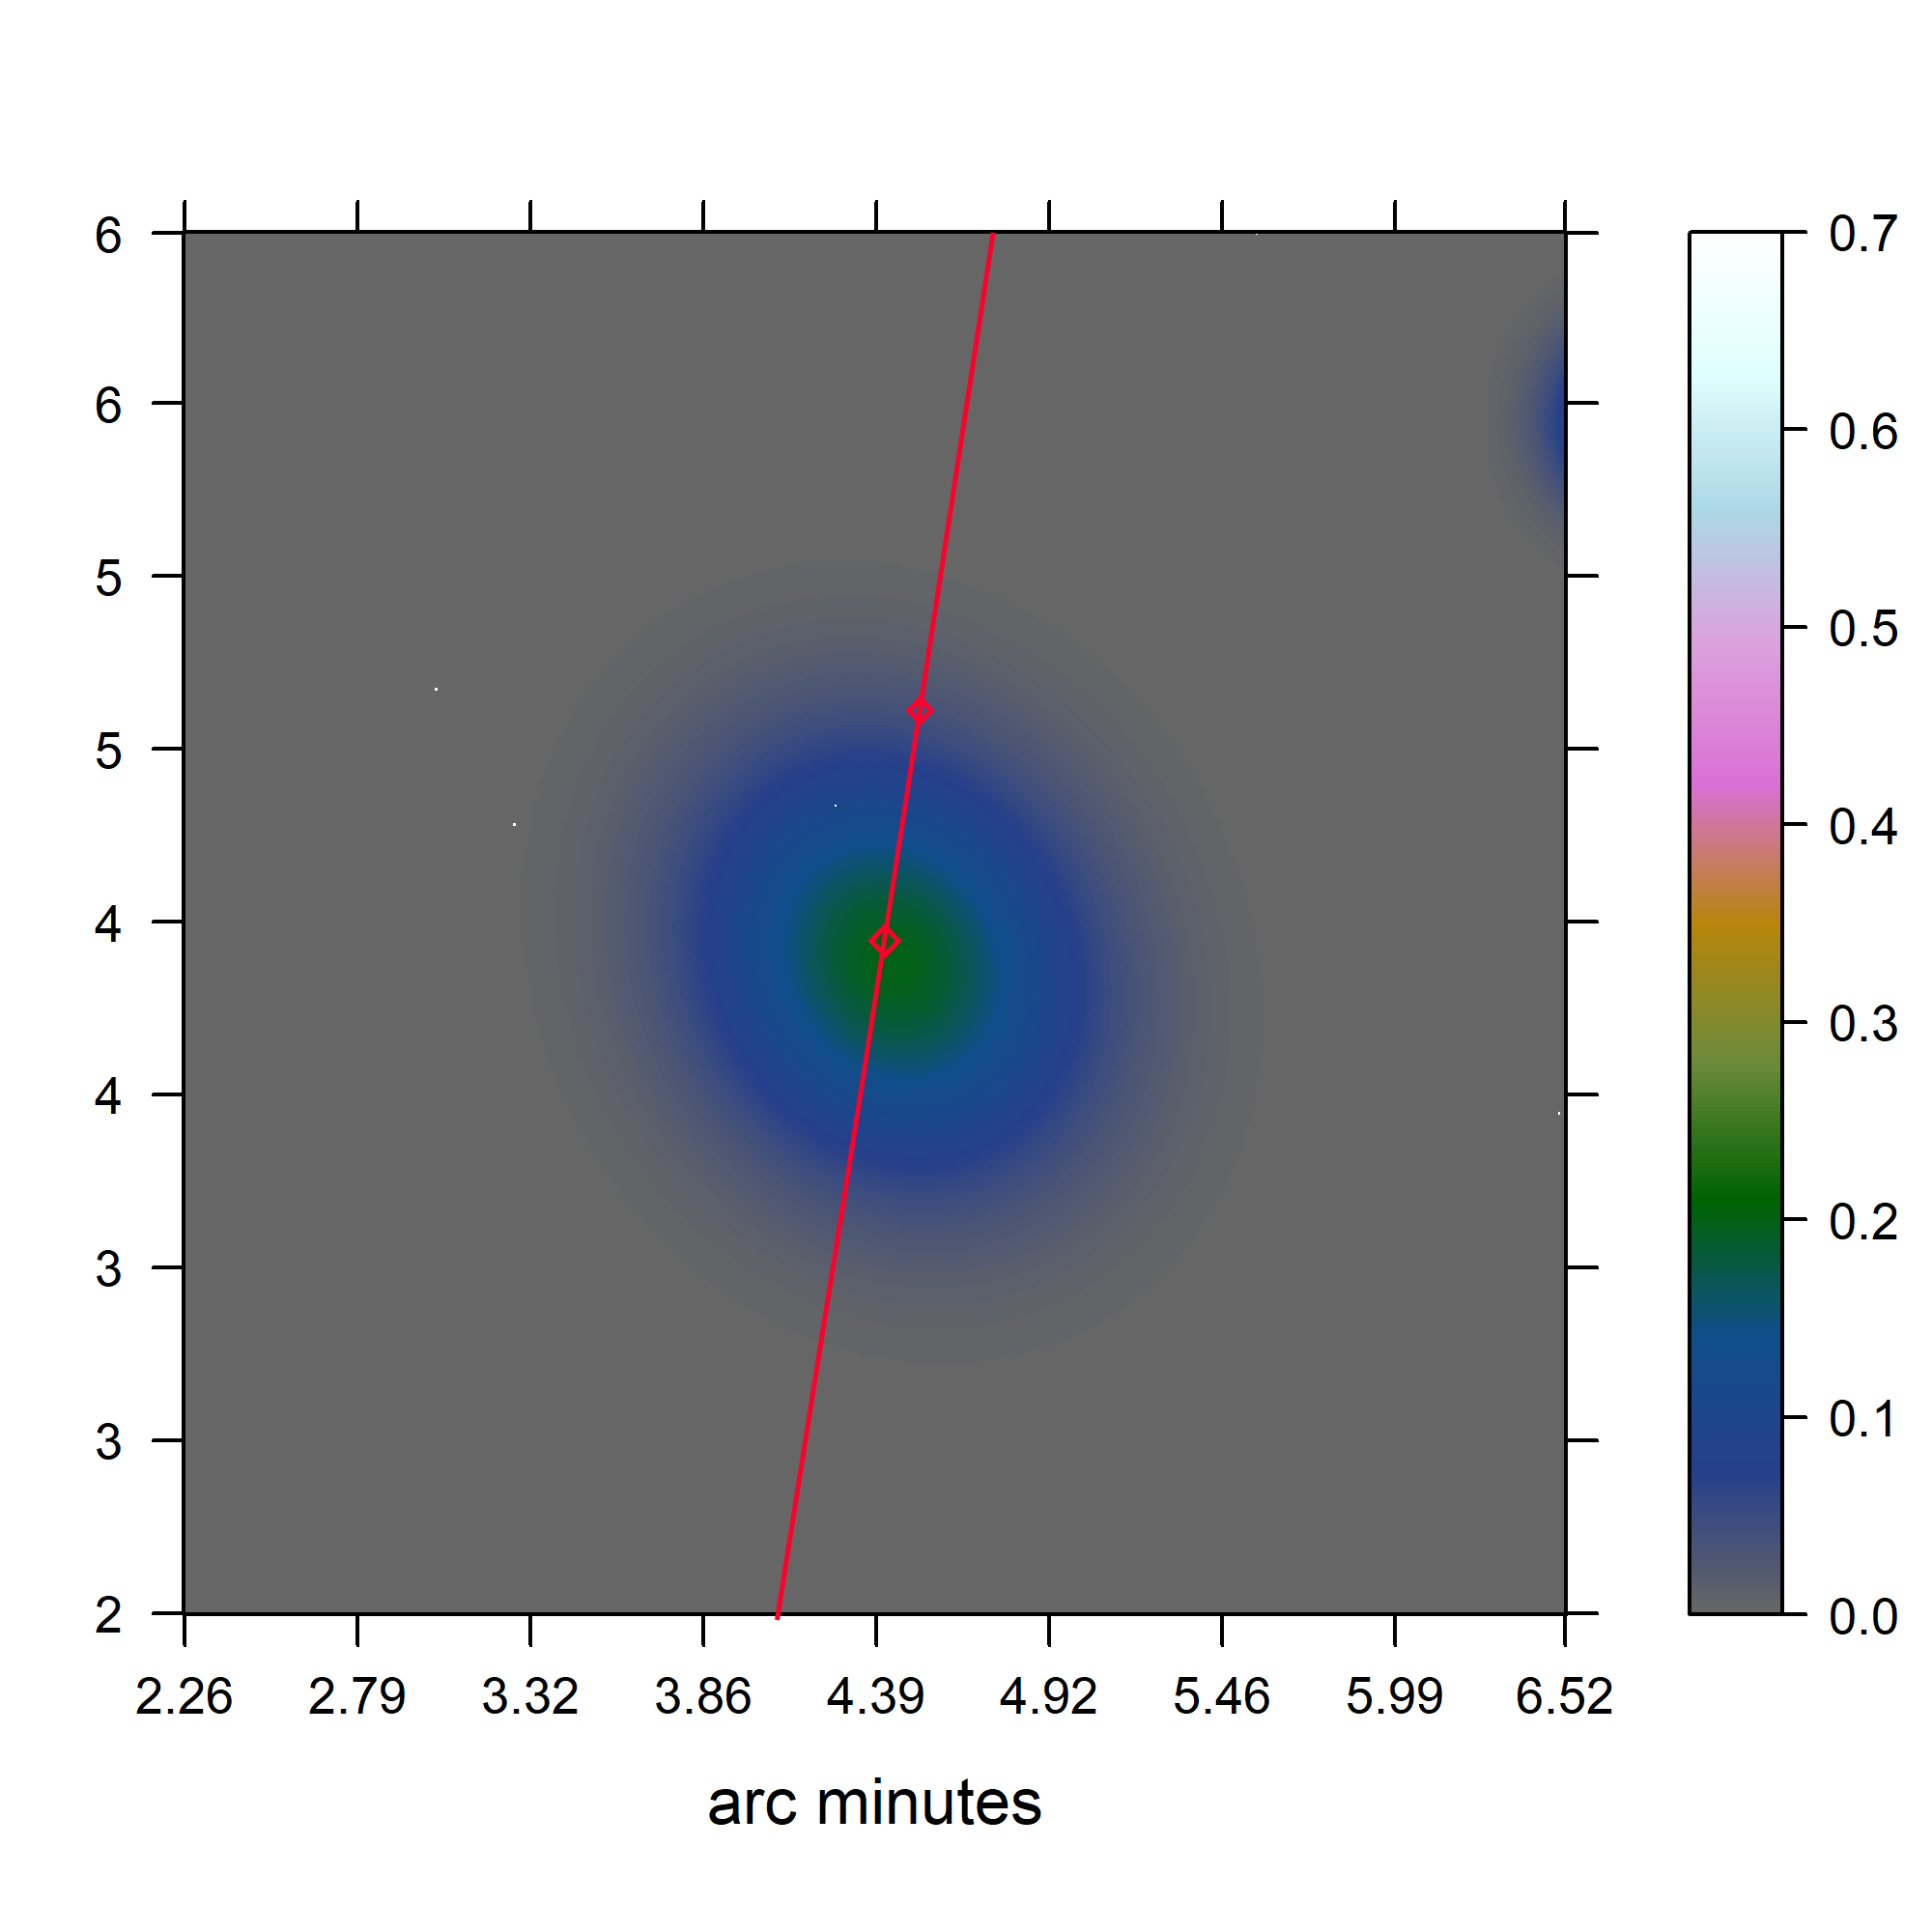
\includegraphics[width=\linewidth, trim={0.4in, 0.9in, 3.2in, 1.8in}, clip]{./chapters/20.results/mixed/mixed_cut_model2_line.png}
		\caption{ground truth}
		\label{results:mixed:cut1:img}
	\end{subfigure}
	\begin{subfigure}[b]{0.6\linewidth}
		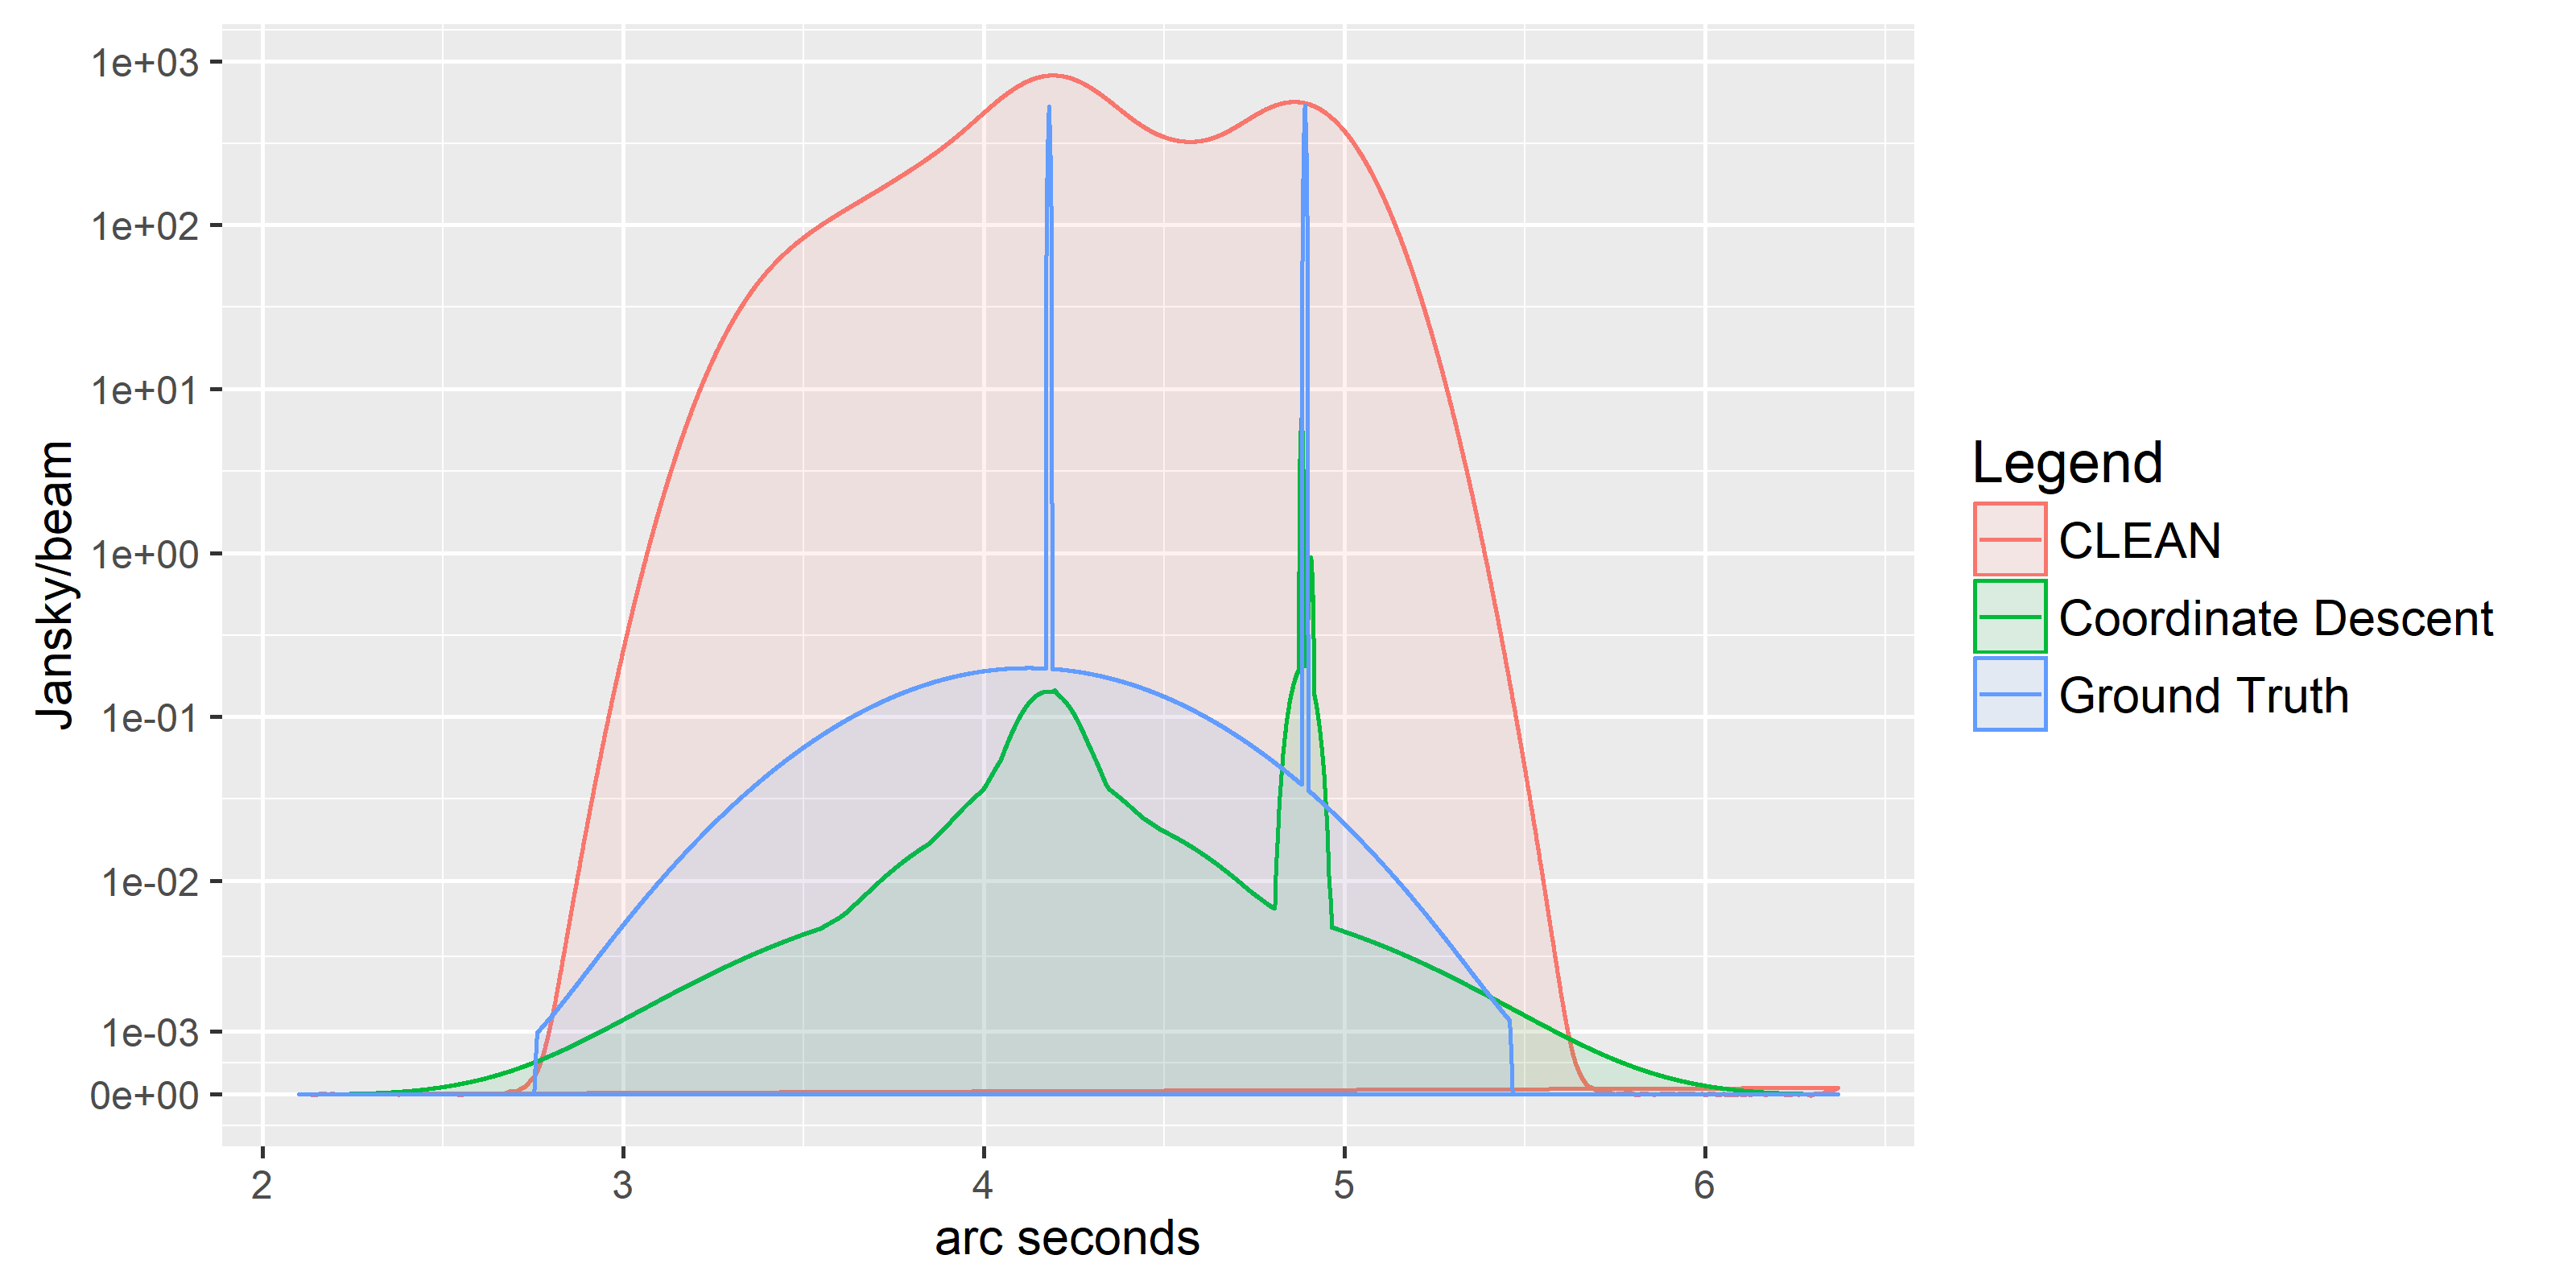
\includegraphics[width=\linewidth, trim={0, 0, 0.2in, 0.2in}, clip]{./chapters/20.results/mixed/mixed_cut2.png}
		\caption{ground truth}
		\label{results:mixed:cut1:profile}
	\end{subfigure}
	\caption{Intensity profile of region 2.}
	\label{results:mixed:cut1:contour}
\end{figure}

More complex source. We see a super resolution and again more accurate flux. Point sources on the other hand, do become problematic. We see one point souce split up in two very narrow peak. When we look at other point sources of figure \ref{results:mixed:points}, we see mixed results. Some point sources are reconstructed as we would wish, with one high peak in the center, locating the point source, and a small starlet artifact which is the low intensity "glow" around it. The first point source is what we would wish for. We show a few failure modes of point source reconstruction. A lower intensity "trail" in the second image and a split into two point sources of images three and four.

\begin{figure}[h]
	\centering
	\begin{subfigure}[b]{0.2\linewidth}
		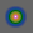
\includegraphics[width=\linewidth]{./chapters/20.results/mixed/problems/point1.png}
	\end{subfigure}
	\begin{subfigure}[b]{0.2\linewidth}
		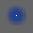
\includegraphics[width=\linewidth]{./chapters/20.results/mixed/problems/point0.png}
	\end{subfigure}
	\begin{subfigure}[b]{0.2\linewidth}
		
\includegraphics[width=\linewidth]{./chapters/20.results/mixed/problems/point2.png}
	\end{subfigure}
	\begin{subfigure}[b]{0.2\linewidth}
		
\includegraphics[width=\linewidth]{./chapters/20.results/mixed/problems/point3.png}
	\end{subfigure}
	\caption{Different point source reconstructions of Coordinate Descent.}
	\label{results:mixed:points}
\end{figure}

problem of an error, since Coordinate Descent should have converged on the two point sources.

Two things could be made to improve it: This project uses the same $\lambda$ for all starlet layers. Girard et al.\cite{girard2015sparse} used a different $\lambda$ for each layer. 

different way of handling positivity. 

The trail issue of point sources can be an artifact of how positivity is handled in our algorithm. 

Starlet reconstruction with negative parts, but leads to a solution with far more non-zero components, [since it has to counter-act the negativity]. The reconstruction \ref{results:mixed:cd} is the result of 244 non-zero, strictly non-negative starlets. Letting the starlet have its negative 'dip' results in a reconstruction with more than ten times the components. 


244 non-zero starlets, 

show the areas


